\documentclass[10pt]{article}

\usepackage[T1]{fontenc}
\usepackage[utf8]{inputenc}
\usepackage{lmodern}
\usepackage[margin=0.85in,top=0.75in,bottom=0.8in]{geometry}
\usepackage{graphicx}
\usepackage{booktabs}
\usepackage{caption}
\usepackage{amsmath}
\usepackage{textcomp}
\usepackage{microtype}
\usepackage{xcolor}
\usepackage[colorlinks=true,linkcolor=black,citecolor=black,urlcolor={blue!50!black}]{hyperref}
\usepackage{enumitem}
\usepackage{fancyhdr}
\usepackage{titlesec}

\raggedbottom
\setlength{\parindent}{0pt}
\setlength{\parskip}{4.5pt}
\captionsetup{font=footnotesize,labelfont=bf,skip=3pt}
\titlespacing*{\section}{0pt}{9pt}{3pt}
\titlespacing*{\subsection}{0pt}{7pt}{2pt}

\pagestyle{fancy}
\fancyhf{}
\renewcommand{\headrulewidth}{0pt}
\fancyfoot[C]{\small\thepage}

% Visible placeholder for anything the repository cannot supply.
\newcommand{\todo}[1]{\textcolor{red}{\textbf{[TODO: #1]}}}

\title{\vspace{-1.5em}\textbf{Benchmarking Protein--Protein Interface Prediction on Experimental versus AlphaFold-Predicted Structures}}
\author{Armeen Shasti-Nazem\thanks{Student, University of Washington,
Seattle, WA, USA. This project was conducted independently, outside of any
course, laboratory, or supervised research program, and does not represent
the University of Washington.}\\[2pt]
\small University of Washington, Seattle, WA, USA\\[1pt]
\small\href{mailto:aashasti@uw.edu}{aashasti@uw.edu}}
\date{\small Draft of \today}

\begin{document}
\maketitle
\thispagestyle{fancy}
\vspace{-2.2em}

\section*{Abstract}

PeSTo is a geometric deep-learning model that predicts protein--protein
interface residues from atomic coordinates, trained only on experimentally
determined structures. Because most protein structures available today are
AlphaFold predictions, we ask whether PeSTo's accuracy transfers to AlphaFold
input. Starting from PDB complexes released after AlphaFold2's training
cutoff and filtered to under @@SEQ_IDENTITY_CUTOFF@@ sequence identity to
PeSTo's own training, validation, and test sequences, we assembled a primary
benchmark set of @@N_LABELED@@ protein chains with both an experimental and
an AlphaFold structure, a validated residue mapping, and interface labels,
and ran PeSTo on each chain's isolated experimental structure and on the
matched AlphaFold model trimmed to the same residue range. Across
@@PRIMARY_N@@ chains with defined metrics, PeSTo's
per-chain area under the precision--recall curve (AUPR) was higher on
experimental input by a median of @@PRIMARY_MEDIAN@@ (95\% CI
@@PRIMARY_CI@@, Wilcoxon $p @@PRIMARY_P@@$), with the same direction in
every subgroup of four pre-specified descriptive splits and under an
alternative buried-surface-area interface definition. The gap was far from
uniform: within AlphaFold's own confidence bands, the pooled AUPR gap shrank
from @@GAP_LOW@@ in the lowest-confidence residues to @@GAP_HIGH@@ in the
highest-confidence residues, and a per-residue regression associated both
AlphaFold confidence (pLDDT) and local structural divergence with how much
each residue's prediction changed between inputs, independently of one
another and of solvent exposure (and, in a post-hoc refit, with
AlphaFold-input predictions lying further from the true label). Chain length was not associated with the
size of the drop. These results describe a modest but consistent,
confidence-linked accuracy cost when applying PeSTo to AlphaFold structures.
The per-residue cost is largest in lower-confidence regions, where interface
residues are over-represented, although most interface residues
(@@FRAC_POS_HIGH_BAND@@) lie in high-confidence (pLDDT $\geq 90$) regions. All
reported relationships are associations, not demonstrated causes.

\section{Introduction}

Protein--protein interactions underlie nearly all cellular processes, from
signal transduction to immune recognition, and the specific residues that form
a binding interface are relevant to understanding disease mutations and to
structure-based drug design \cite{zhang2024}. Determining an interface
experimentally, by solving the structure of a complex, remains slow relative to
the scale of the problem: the Protein Data Bank (PDB) holds on the order of
$2\times10^5$ structures, while the AlphaFold Protein Structure Database now
provides predicted structures for over $2\times10^8$ sequences
\cite{jumper2021,varadi2024}. Several geometric deep-learning methods now
predict interface residues directly from a single protein's three-dimensional
coordinates, without requiring a solved complex: PeSTo represents atoms by
element and position alone \cite{krapp2023}, and ScanNet extracts learned
geometric and biochemical descriptors \cite{tubiana2022}. These models are
trained on experimentally determined structures, and applying them to
AlphaFold predictions implicitly assumes the predicted geometry is close
enough to the true structure that the model's learned decision boundary still
applies.

That assumption is worth checking directly. AlphaFold reports a per-residue
confidence score, pLDDT. Its documentation states that a pLDDT above 70
usually corresponds to a correct backbone prediction, while regions below 50
are often flexible or intrinsically disordered \cite{afdbplddt}. Interface
residues are over-represented among low-confidence residues: in the dataset
analyzed here, the interface base rate is @@BASE_RATE_LOW@@ among residues
with pLDDT below 50 versus @@BASE_RATE_HIGH@@ among those at or above 90
(Table~\ref{tab:bands}). Even confidently predicted regions deviate
measurably from experimental structures: Terwilliger et al.\ report median
inter-atomic distance deviations, within regions of pLDDT above 70, of about
0.1\,\r{A} for nearby atom pairs rising to about 0.7\,\r{A} for pairs
roughly 50\,\r{A} apart \cite{terwilliger2024}. Yuan et al.\ reported that
PeSTo's median per-protein AUPR on PeSTo's own protein--protein test set fell
from 0.797 with experimental input (the value reported by PeSTo's authors)
to 0.691 with ESMFold-predicted input \cite{yuan2024,lin2023}. ESMFold is a
protein-language-model-based structure predictor distinct from AlphaFold,
so this is a substantial drop but not a direct measurement of AlphaFold
specifically, whose error characteristics differ from ESMFold's.

This paper reports a matched, AlphaFold-specific benchmark of PeSTo together
with an error analysis of where any accuracy gap occurs. We ask two
questions: (1) how much does PeSTo's interface-prediction accuracy change when
the input is an AlphaFold model of a chain rather than that chain's own
experimental structure, holding the chain and the ground-truth interface
fixed; and (2) is that change associated with AlphaFold's own confidence score
and with the local geometric divergence between the two structures. Both
analyses followed written analysis plans fixed before they were run on real
predictions (Section~\ref{sec:prespec} describes exactly what was fixed when).
PeSTo's authors themselves applied it to 7,464 high-quality human AlphaFold
DB models, selected by pLDDT and PAE, and reported that agreement with
predicted yeast complexes improved in higher-quality model regions
\cite{krapp2023}. This study extends that work and Yuan et al.'s ESMFold
benchmark to a controlled, AlphaFold-specific comparison on matched
experimental structures, with a paired error analysis; it is not the first
study to raise this general concern.

\section{Methods}

\subsection{Dataset construction}

Candidate protein chains were drawn from X-ray crystal structures in the PDB
released after @@RELEASE_DATE_CUTOFF@@, AlphaFold2's own training-data
cutoff, so that the experimental structures used here were not part of
AlphaFold2's training data (see Limitations regarding the templates used to
generate the AlphaFold DB models). Candidates were restricted to entries at
or better than @@RESOLUTION_CUTOFF@@\,\r{A} resolution with no nucleic-acid
polymer entities, complexes of at most @@MAX_PROTEIN_ENTITIES@@ distinct
protein entities (excluding assemblies too large for a single well-defined
pairwise interface, e.g.\ viral capsids), and chains whose polymer entity
sequence is at least @@MIN_CHAIN_LENGTH@@ residues long (the entity's full
expressed/construct sequence, not the count of residues actually resolved in
the deposited coordinates, which is often substantially smaller). Each
chain's UniProt accession from the RCSB Data API was cross-checked against
the SIFTS \cite{velankar2013} bulk chain-to-UniProt mapping (release
header: @@SIFTS_BULK_RELEASE@@). This search returned @@N_ENTRIES@@ PDB
entries and @@N_CHAINS@@ candidate protein chains (Fig.~\ref{fig:attrition}).
Redundant chains were then collapsed with MMseqs2 \cite{steinegger2017}
(version @@MMSEQS_VERSION@@) \texttt{easy-cluster} at
\texttt{-{}-min-seq-id} @@SEQ_IDENTITY_CUTOFF@@ and \texttt{-c}
@@CLUSTER_MIN_COVERAGE@@ with \texttt{-{}-cov-mode 0} (the alignment must cover
at least @@CLUSTER_MIN_COVERAGE@@ of both sequences), all other parameters at
their defaults (greedy set-cover clustering, sensitivity 4, E-value
$10^{-3}$), to @@N_CLUSTERS@@ non-redundant representatives; each cluster's
representative is its best-resolution member, then its longest, then the
first by PDB and chain identifier.

Because PeSTo was trained on essentially all biological assemblies in the PDB,
filtering by exact PDB identifier is not sufficient: a chain released after
2018 can still be a close sequence homolog of something PeSTo has already seen
under a different identifier. Each representative was therefore searched with
MMseqs2 \texttt{easy-search} against the union of PeSTo's published training,
validation, and test sequence sets (same version; \texttt{-{}-min-seq-id}
@@SEQ_IDENTITY_CUTOFF@@, \texttt{-c} @@CLUSTER_MIN_COVERAGE@@,
\texttt{-{}-cov-mode 0}, default sensitivity 5.7 and E-value $10^{-3}$;
identity is MMseqs2's identical positions over alignment length).
@@OVERLAP_PCT@@ of representatives had a hit at or above
@@SEQ_IDENTITY_CUTOFF@@ identity and were treated as leakage. The
leakage-free candidate set carried forward into the rest of the pipeline is
the @@N_LEAKAGE_FREE@@ representatives below this threshold; not all of them
survive the remaining processing steps below, which is why this paper
distinguishes the leakage-free candidate set (@@N_LEAKAGE_FREE@@) from the
smaller primary benchmark set that is actually analyzed in
Section~\ref{sec:results} (@@N_LABELED@@, defined below).

For each leakage-free representative, the PDBe ``updated'' mmCIF file
(downloaded @@PDBE_DOWNLOAD_DATE@@) and the corresponding AlphaFold DB model
(queried through the AlphaFold DB prediction API and downloaded
@@AF_DOWNLOAD_DATE@@) were retrieved; @@N_STRUCTURES@@ representatives had
both. The rest had no AlphaFold DB entry for their UniProt accession
(@@N_AF_ABSENT@@), were split into fragments in AlphaFold DB
(@@N_AF_FRAGMENTED@@), or had an AlphaFold DB sequence that did not match
the UniProt sequence (@@N_AF_SEQ_MISMATCH@@). Every AlphaFold model in the
primary benchmark set is AlphaFold DB model version @@AF_MODEL_VERSIONS@@,
generated by the ``@@AF_TOOL_USED@@'' (model creation date
@@AF_MODEL_CREATED_RANGE@@ in the API metadata). AlphaFold DB also serves
third-party community models under the same per-accession query as official
AlphaFold2 predictions; these were identified from the API metadata's
provider field and excluded (@@N_NONOFFICIAL_AF@@ representatives, provider
@@NONOFFICIAL_PROVIDERS@@, e.g.\ ColabFold models), since they do not carry
AlphaFold2's training-cutoff guarantee.

Residue numbering between the experimental structure and the AlphaFold model
(which uses UniProt numbering) was mapped residue by residue using the SIFTS
cross-references embedded in each PDBe updated mmCIF file, falling back to a
pairwise sequence alignment when SIFTS was unavailable or failed a
$\geq$@@MAPPING_VALIDATION_IDENTITY@@ residue-identity validation check.
Chains were excluded if neither method passed validation
(@@N_VALIDATION_EXCL@@) or if fewer than @@MIN_MAPPED_COVERAGE@@ of the
chain's observed residues mapped to a position within the AlphaFold model
(@@N_COVERAGE_EXCL@@). @@N_MAPPED@@ representatives obtained a validated
mapping. Of the @@N_LABELED@@ chains in the final primary set,
@@N_SIFTS_MAPPED@@ used the SIFTS mapping and @@N_FALLBACK_MAPPED@@ the
fallback alignment; @@N_NONIDENTICAL@@ contain at least one residue that
differs from the AlphaFold model's sequence (minimum identity
@@MIN_MAPPED_IDENTITY@@), typically engineered point mutations.

Ground-truth interface residues were computed from coordinates in the
depositor-annotated biological assembly -- not the raw crystallographic
asymmetric unit, which is dominated by crystal-packing contacts unrelated to
biological interfaces, and not the PISA assembly-annotation service
\cite{krissinel2007}, which has no practical batch interface for a set this
size. For each chain, the first author-determined assembly containing it
was used (otherwise the first listed assembly containing it; the asymmetric
unit itself only for entries that define no assembly). A residue is an
interface residue if any of its heavy atoms lies within
@@INTERFACE_DISTANCE_CUTOFF@@\,\r{A} of any heavy atom of a standard or
modified amino-acid residue on another chain of that assembly, including
symmetry-generated copies; ligands, ions, waters, and nucleic acids are not
partners. Alternate conformations were resolved per atom by highest
occupancy, and hydrogens were ignored throughout. A second,
buried-surface-area--based definition (loss of at least
@@SASA_BURIAL_CUTOFF@@\,\r{A}$^2$ of solvent-accessible surface area when
the protein partners are added) was retained as a robustness check on the
labeling choice; SASA was computed with Biotite's Shrake--Rupley
implementation \cite{kunzmann2018,shrake1973} (version @@BIOTITE_VERSION@@,
ProtOr radii \cite{tsai1999}, probe radius @@SASA_PROBE@@\,\r{A},
@@SASA_POINTS@@ points per atom). Chains were excluded at this step if their
assembly contained no protein partner (@@N_NO_PARTNER@@) or no residue met
the interface criterion (@@N_ZERO_INTERFACE@@), @@N_LABEL_EXCL@@ in total. The remaining @@N_LABELED@@
representatives form the primary benchmark set analyzed in
Section~\ref{sec:results}; a full list is provided as Supplementary
Table~S1 (Code and Data Availability).

\begin{figure}[t]
\centering
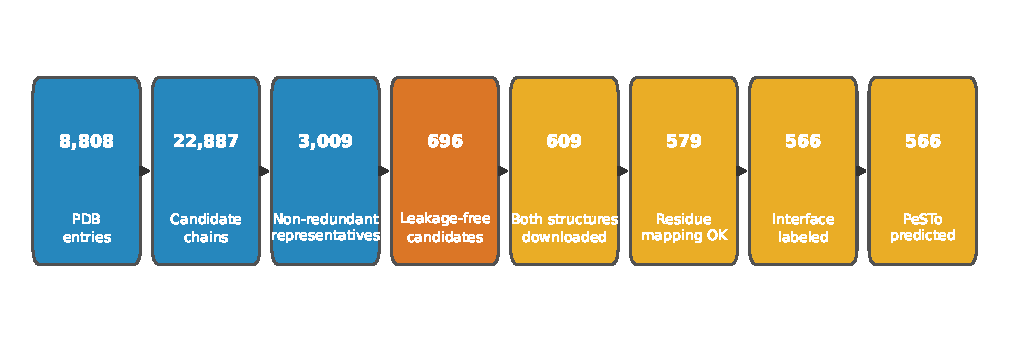
\includegraphics[width=\textwidth]{figures/fig1_attrition.pdf}
\caption{Dataset construction: candidate PDB chains are reduced by
redundancy clustering, sequence-level leakage filtering against PeSTo's own
training/validation/test data, structure availability, residue-mapping
validation, and interface labeling, to the @@N_PREDICTED@@-chain primary
benchmark set. Counts from ``Leakage-free candidates'' onward are for the
leakage-filtered chains only.}
\label{fig:attrition}
\end{figure}

\subsection{Inference}

The pretrained PeSTo model (repository commit @@PESTO_COMMIT@@, checkpoint
@@PESTO_CHECKPOINT@@, which takes atomic elements and coordinates as input)
was run on each of the @@N_PREDICTED@@ primary-set chains in two input forms.
The experimental input (\emph{exp}) is the chain's own heavy atoms from the
PDBe mmCIF file -- every observed polymer residue of the chain, with other
chains, waters, ligands, and ions removed, alternate conformations resolved
as above, and modified residues (e.g.\ selenomethionine) kept as deposited;
missing atoms were not rebuilt. The AlphaFold input (\emph{af\_trimmed}) is
the AlphaFold model's heavy atoms for every residue between the first and
last mapped UniProt position, inclusive; it therefore also contains residues
inside that range that are unresolved in the experimental structure, while
the experimental input contains any observed residues that do not map to
UniProt (e.g.\ expression tags). Both runs used the chain in isolation, with
no partner structure present, matching how an interface predictor would be
applied to a single AlphaFold model in practice. We used PeSTo's
protein--protein interface output (channel 0, sigmoid-transformed). All
metrics are computed only on the residues present in both inputs and mapped
between them, so each chain is scored on an identical residue set and against
identical labels for both inputs.

\subsection{Derived structural features}
\label{sec:features}

Relative solvent accessibility (RSA) is the residue's SASA in the isolated
experimental chain (its bound conformation with partners removed) divided by
the theoretical maximum of Tien et al.\ \cite{tien2013}; ``surface'' residues
are those with RSA $\geq @@SURFACE_RSA_THRESHOLD@@$. Secondary structure
(helix, strand, coil) was assigned from the experimental C$\alpha$ trace by
P-SEA \cite{labesse1997} as implemented in Biotite (DSSP was not available
in the computing environment). pLDDT was read from the AlphaFold model's
B-factor column. A residue's local C$\alpha$ RMSD uses the mapped residues
whose experimental C$\alpha$ lies within @@LOCAL_RMSD_RADIUS@@\,\r{A} of its
own (itself included; at least @@LOCAL_RMSD_MIN_NEIGHBORS@@ required), with a
separate Kabsch superposition of that neighborhood's C$\alpha$ atoms and the
RMSD taken over the same neighborhood, so that structural motion elsewhere in
a multi-domain chain is not mistaken for local error at a given residue.

A chain is \emph{geometrically flagged} if, after one global Kabsch
superposition of all its mapped C$\alpha$ atoms onto the AlphaFold model's,
at least @@GEO_RUN@@ consecutive mapped residues (in UniProt order) are more
than @@GEO_FAR@@\,\r{A} apart. This check was built to catch residue
mappings that pass sequence validation but do not correspond in 3D; in
practice it also flags genuine large-scale conformational differences, such
as domain rearrangements.

\subsection{Pre-specified analysis plans}
\label{sec:prespec}

Sections~\ref{sec:benchmark} and~\ref{sec:error} follow analysis plans
written into the project's design document before each analysis was run on
real predictions. These plans are pre-specified, not publicly pre-registered,
and the record of their timing is limited in one specific way. The original
project plan (committed 2026-09-16, \texttt{ac34866}, before any data were
downloaded) already specified the paired Wilcoxon test with a bootstrap CI on
per-chain AUPR, pLDDT bands at @@PLDDT_BANDS@@, local RMSD, RSA, and
secondary structure as covariates, and flagging of predictors with VIF above
@@VIF_THRESHOLD@@. The detailed plans (exact endpoints, strata, thresholds,
and regression specification) were written later and committed to version
control in the same commits as the corresponding results (\texttt{f289b6b}
and \texttt{8db13d4}). That they preceded the results therefore rests on the
author's own records, not on an independent timestamp. The error-analysis
plan was written after the benchmark results were known. It also changed the
original plan's regression outcome (a binary prediction-error indicator,
modeled by logistic regression) to the continuous prediction shift described
below, before any error-analysis feature was computed.

\textbf{Post-hoc analyses added after review.} Five further analyses were
chosen after all of the above results were known, in response to peer
review (code: \texttt{src/analysis/posthoc\_review.py}). They are
exploratory, are reported together in Section~\ref{sec:review} (except the
paired F1 bootstrap, reported with the filtering analysis it tests), and do
not replace any pre-specified result. (1) \emph{Template window:} each chain's
PDB release date was compared with its AlphaFold DB model's creation date,
and the primary endpoint repeated on the chains released on or after that
date, which cannot have served as templates for their own models. (2)
\emph{Signed error:} the regression design above was refitted with
$|p_{\mathrm{AF}} - y| - |p_{\mathrm{exp}} - y|$ as the outcome, where $y$
is the true label (positive when the AlphaFold-input prediction is further
from the truth), and $R^2$ is reported for both outcomes. (3) \emph{Paired
F1 bootstrap} for Section~\ref{sec:filtering}: the change in F1 between the
smallest and largest pLDDT cutoff, and the change in the
experimental-vs.-AlphaFold F1 gap, with both cutoffs evaluated on the same
resampled chains (@@BAND_BOOTSTRAP_N@@ resamples). (4) \emph{Pooled vs.\
per-chain gap:} pooled AUPR recomputed after removing the
@@PV_TRIM_PCT@@ of chains with the largest per-chain drops, and after
replacing each chain's scores by their within-chain percentile rank, which
removes differences in score calibration between chains. (5) \emph{Flag
audit:} mapping method and identity of geometrically flagged vs.\ unflagged
chains, and a per-chain listing of residues with local RMSD above
@@EX_THRESH@@\,\r{A}.

\textbf{Benchmark (Section~\ref{sec:benchmark}).} Primary and secondary
endpoints are the paired per-chain difference (experimental minus
AlphaFold-trimmed) in AUPR and ROC-AUC respectively, restricted to chains
where both metrics are defined (excluding chains whose scored residues are
single-class). Each was tested with a two-sided Wilcoxon signed-rank test
($\alpha = 0.05$) and a 95\% percentile bootstrap CI on the median difference
(@@BOOTSTRAP_N@@ resamples of chains, not residues, with replacement, since
residues within one chain are not independent observations; fixed seed
@@PHASE7_SEED@@). Pooled-residue AUPR and ROC-AUC were reported for each
input. Four binary splits were specified as descriptive strata, reported
side by side with $n$, not as additional hypothesis tests, and not corrected
for multiple comparisons: homomeric vs.\ heteromeric partner, interface
fraction below vs.\ at or above @@INTERFACE_FRACTION_THRESHOLD@@,
geometrically flagged vs.\ not, and all residues vs.\ surface residues
only. A robustness check repeats the primary endpoint with the
buried-surface-area label.

\textbf{Error analysis (Section~\ref{sec:error}).} pLDDT confidence bands are
fixed at @@PLDDT_BANDS@@ (AlphaFold's own convention). Pooled AUPR/ROC-AUC
are computed for both inputs within each band, with chain-resampled 95\%
percentile bootstrap CIs (@@BAND_BOOTSTRAP_N@@ resamples per band, fewer than
the benchmark's @@BOOTSTRAP_N@@ because each draw here recomputes a full
pooled metric over tens of thousands of residues rather than a cheap scalar;
fixed seed @@PHASE8_SEED@@). A per-residue ordinary-least-squares regression
relates the absolute prediction shift, $|p_{\mathrm{AF}} -
p_{\mathrm{exp}}|$, to standardized pLDDT, standardized local C$\alpha$ RMSD,
standardized RSA, and secondary-structure class (coil as reference). Standard
errors are cluster-robust (CRV1), clustered by chain, and variance inflation
factors (VIF) are reported for each predictor (flagged above
@@VIF_THRESHOLD@@, since pLDDT and local RMSD both reflect
AlphaFold-vs-experimental divergence and were expected to correlate).
Descriptive analyses of chain length and of the geometrically flagged chains
were specified as associations to be reported, not confirmatory tests. In
the results, $p$-values below $@@P_FLOOR@@$ are reported only as that bound.

\textbf{Which chains enter which analysis.} Per-chain analyses (the paired
endpoints, the descriptive strata, and the chain-length and flagged-chain
comparisons) use the @@PRIMARY_N@@ chains for which per-chain metrics are
defined. Residue-level analyses (pooled metrics, pLDDT bands, the shift
regression, and Section~\ref{sec:filtering}) use every scored residue of all
@@N_LABELED@@ chains, including the @@EXCL_RES@@ residues
(@@EXCL_RES_PCT@@ of the pooled total) of the @@N_EXCLUDED@@ single-class
chains described in Section~\ref{sec:benchmark}.

\section{Results}
\label{sec:results}

\subsection{Benchmark: experimental versus AlphaFold-trimmed input}
\label{sec:benchmark}

Of the @@N_LABELED@@ primary-set chains, @@N_EXCLUDED@@ (@@EXCLUDED_PCT@@)
were excluded from every per-chain comparison because every scored residue
in the chain was labeled interface (these chains have only
@@EXCL_MIN_N@@--@@EXCL_MAX_N@@ scored residues), leaving no non-interface
residues against which to compute ROC-AUC or AUPR; the remaining
@@PRIMARY_N@@ chains form the primary comparison.

PeSTo was more accurate on experimental input than on the matched
AlphaFold-trimmed input: the median paired AUPR difference was
@@PRIMARY_MEDIAN@@ (95\% CI @@PRIMARY_CI@@, Wilcoxon $p @@PRIMARY_P@@$), and
the paired ROC-AUC difference showed the same pattern (median
@@ROC_MEDIAN@@, CI @@ROC_CI@@, $p @@ROC_P@@$). The direction was not
universal: AlphaFold input gave the higher AUPR for @@N_AF_BETTER@@ of
@@PRIMARY_N@@ chains (@@PCT_AF_BETTER@@), experimental input for
@@N_EXP_BETTER@@, with @@N_TIE@@ tie. Pooling all @@POOLED_N@@ scored
residues (interface base rate @@POOLED_BASE_RATE@@) rather than comparing
per chain gives AUPR @@POOLED_AUPR_EXP@@ on experimental input versus
@@POOLED_AUPR_AF@@ on AlphaFold input (pooled ROC-AUC @@POOLED_ROC_EXP@@
vs.\ @@POOLED_ROC_AF@@). Both inputs are far above the base rate, so both
are informative, but the pooled AUPR gap (@@POOLED_AUPR_DIFF@@) is
noticeably larger than the per-chain median gap; Section~\ref{sec:error}
returns to this. Replacing the distance-based interface label with the
buried-surface-area label gives essentially the same result (median
@@ROBUST_MEDIAN@@, CI @@ROBUST_CI@@, $p @@ROBUST_P@@$), so the finding is not
an artifact of the distance-cutoff label definition. The gap also persists
among chains that cannot have served as templates for their own AlphaFold
models (post-hoc, Section~\ref{sec:review}).


\begin{figure}[t]
\centering
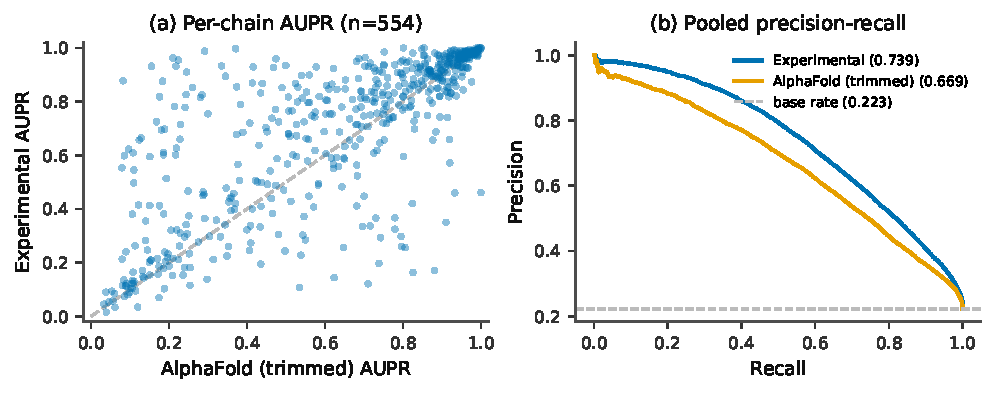
\includegraphics[width=\textwidth]{figures/fig2_phase7_primary.pdf}
\caption{(a) Per-chain AUPR, experimental vs.\ AlphaFold-trimmed input; most
chains sit near the identity line with a tilt toward experimental input, and a
right-skewed tail where AlphaFold input costs noticeably more accuracy. (b)
Precision--recall curves pooling every scored residue in the primary set,
for each input, against the pooled interface base rate.}
\label{fig:phase7primary}
\end{figure}

Across the four pre-specified descriptive splits (Fig.~\ref{fig:strata}),
every subgroup showed the same direction of effect, with medians from
@@STRATA_LO_VALUE@@ ($n = @@STRATA_LO_N@@$, @@STRATA_LO_LABEL@@) to
@@STRATA_HI_VALUE@@ ($n = @@STRATA_HI_N@@$, @@STRATA_HI_LABEL@@), and no
subgroup's bootstrap CI included zero. (The all-residues arm of the
residue-scope split is the primary endpoint itself, so
@@N_DESCRIPTIVE_SUBGROUPS@@ distinct subgroups are shown alongside it.) As
pre-specified, these are descriptive comparisons and are not interpreted as
further hypothesis tests. The gap is therefore not confined to one kind of
chain, though its size varies noticeably. It is largest among the minority
of geometrically flagged chains, those whose AlphaFold model and
experimental structure disagree over a long contiguous stretch after
superposition (Section~\ref{sec:features}).

\begin{figure}[t]
\centering
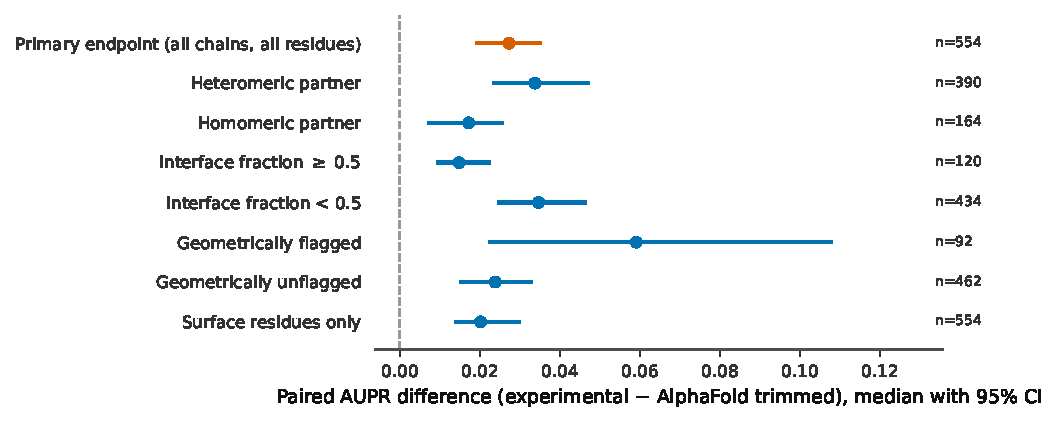
\includegraphics[width=\textwidth]{figures/fig3_phase7_strata.pdf}
\caption{Paired AUPR difference (median, 95\% chain-resampled bootstrap CI)
for the primary endpoint and the subgroups of the four pre-specified
descriptive splits. The all-residues subgroup is identical to the primary
endpoint and is shown once. All intervals lie on the same side of zero.}
\label{fig:strata}
\end{figure}

\subsection{Error analysis: what the gap is associated with}
\label{sec:error}

Stratifying every scored residue by AlphaFold's own pLDDT confidence band
(Fig.~\ref{fig:bands}, Table~\ref{tab:bands}) shows the AUPR gap shrinking
monotonically as confidence increases, from @@GAP_LOW@@ in the lowest band to
@@GAP_HIGH@@ in the highest -- roughly a @@GAP_RATIO@@-fold reduction
(computed from unrounded values) -- with the same pattern in ROC-AUC. Every
band cleared the minimum-residue reporting threshold with no undefined
bootstrap draws.

\begin{figure}[t]
\centering
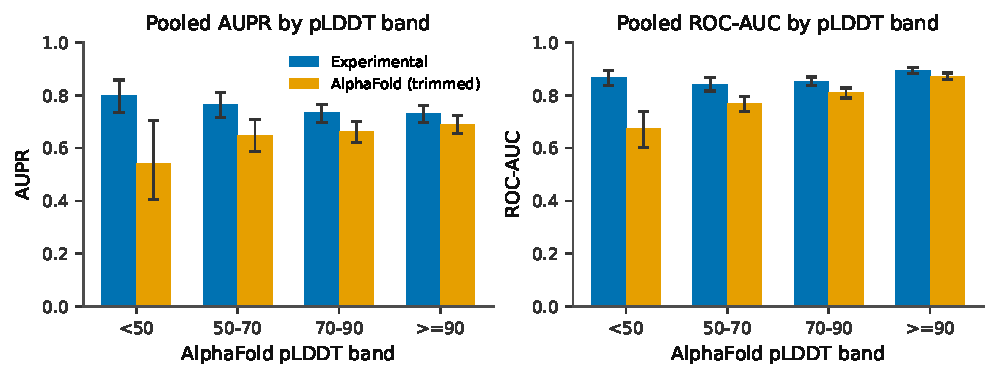
\includegraphics[width=\textwidth]{figures/fig4_phase8_bands.pdf}
\caption{Pooled AUPR and ROC-AUC by AlphaFold pLDDT confidence band, both
inputs, with 95\% chain-resampled bootstrap CIs. The experimental-vs.-AlphaFold
gap is largest in AlphaFold's least confident residues and smallest in its
most confident ones.}
\label{fig:bands}
\end{figure}

\begin{table}[t]
\centering
\small
@@BAND_TABLE@@
\caption{Pooled ROC-AUC and AUPR by pLDDT band, both inputs, with 95\%
chain-resampled bootstrap CIs.}
\label{tab:bands}
\end{table}

A per-residue regression of the absolute prediction shift on standardized
pLDDT, local RMSD, RSA, and secondary structure (Fig.~\ref{fig:regression},
Table~\ref{tab:regression}; $n = @@REG_N@@$ of the @@POOLED_N@@ pooled
residues,\footnote{@@REG_N_DROPPED@@ residue was excluded for a missing RSA
value: a single non-standard N-terminal residue whose chemical component has
no reference maximum accessible surface area in the table of Tien et
al.\ \cite{tien2013}. It was logged during interface labeling and is not
otherwise informative for this regression.} @@REG_CLUSTERS@@ chains as
clusters, cluster-robust standard errors) finds pLDDT
(coefficient @@PLDDT_COEF@@, $p @@PLDDT_P@@$) and local RMSD (coefficient
@@RMSD_COEF@@, $p @@RMSD_P@@$) each independently associated with the size of
the shift in the expected direction -- higher confidence is associated with a
smaller shift, larger local structural divergence with a larger one -- after
controlling for the other and for RSA. RSA had the strongest association of
any predictor (coefficient @@RSA_COEF@@, $t = @@RSA_T@@$, $p @@RSA_P@@$,
versus $|t| = @@PLDDT_T@@$ for pLDDT and @@RMSD_T@@ for local RMSD):
predictions for more exposed residues change more between inputs. No
predictor's variance inflation factor exceeded @@VIF_THRESHOLD@@ (maximum
@@MAX_VIF@@): although both are proxies for AlphaFold-vs-experimental
divergence, pLDDT and local RMSD are only mildly collinear here and each
retains independent explanatory power. The shift measures how much a
prediction moves between inputs, not whether it moves toward or away from
the true label, and the regression explains only a small part of its
variance ($R^2 = @@SHIFT_R2@@$); Section~\ref{sec:review} refits the same
design on the signed error. Binned by local-RMSD decile, the mean
absolute prediction shift changes little across the lowest deciles and
rises over the upper ones, most steeply in the top decile
(Fig.~\ref{fig:regression}a).





\begin{figure}[t]
\centering
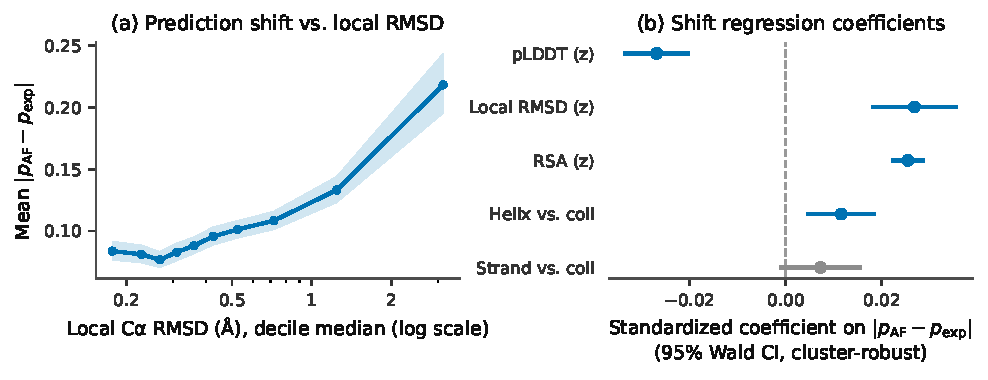
\includegraphics[width=\textwidth]{figures/fig5_phase8_regression.pdf}
\caption{(a) Mean absolute prediction shift in each decile of local
C$\alpha$ RMSD (equal numbers of residues per decile), plotted at the
decile's median local RMSD on a log scale, with chain-resampled 95\% CIs.
(b) Standardized coefficients (95\% Wald CI, cluster-robust) from the
per-residue shift regression; grey markers did not reach $p < 0.05$.}
\label{fig:regression}
\end{figure}

\begin{table}[t]
\centering
\small
@@REGRESSION_TABLE@@
\caption{Regression of $|p_{\mathrm{AF}}-p_{\mathrm{exp}}|$ on standardized
predictors, cluster-robust standard errors by chain.
Reference category: secondary structure = coil.}
\label{tab:regression}
\end{table}



Two pre-specified descriptive analyses addressed possible confounds. First,
per-chain AUPR drop showed no meaningful association with chain length
(Spearman $\rho = @@RHO@@$, 95\% CI @@RHO_CI@@, $p @@RHO_P@@$). This
contradicts the analysis plan's stated expectation that chain length would
explain why the pooled AUPR gap (@@POOLED_AUPR_DIFF@@) exceeds the per-chain
median gap (@@PRIMARY_MEDIAN@@). The drop distribution is instead
right-skewed (unweighted mean @@UNWEIGHTED_MEAN_DROP@@ vs.\ median
@@UNWEIGHTED_MEDIAN_DROP@@), and weighting the mean by chain length barely
moves it (@@WEIGHTED_MEAN_DROP@@). A minority of chains with unusually large
drops pull the mean above the median; long chains in general do not
(Section~\ref{sec:review} examines how much of the pooled-vs.-median
difference this tail accounts for).

Second, the @@FLAGGED_N@@ geometrically flagged chains differ from
the remaining @@UNFLAGGED_N@@ on every measure in Table~\ref{tab:flagged}
except interface fraction. Their larger global C$\alpha$ distances follow
from how the flag is defined, and their larger local RMSD ($p @@FLAGGED_RMSD_P@@$) is closely related.
The evidence that does not depend on the flag's definition is AlphaFold's own
confidence: flagged chains have substantially lower mean pLDDT
($p @@FLAGGED_PLDDT_P@@$), which is consistent with genuine
AlphaFold-vs-experimental divergence rather than a mapping artifact, though
it does not rule out the latter for individual chains. Flagged chains are
also longer, consistent with (but not evidence for) domain rearrangement in
multi-domain chains. A post-hoc audit of their residue mappings is in
Section~\ref{sec:review}.

\begin{table}[t]
\centering
\small
@@FLAGGED_TABLE@@
\caption{Geometrically flagged vs.\ unflagged primary-set chains
(two-sided Mann--Whitney $U$ test).}
\label{tab:flagged}
\end{table}

Figure~\ref{fig:structure} illustrates these results on a single chain
(PDB @@EX_PDB_ID@@, chain @@EX_CHAIN_ID@@, UniProt @@EX_UNIPROT@@,
@@EX_N@@ residues), chosen because its AUPR drop (@@EX_DROP@@) sits close to
the primary endpoint's median. PeSTo's experimental-input predictions
(AUPR @@EX_AUPR_EXP@@) track the true interface patch more tightly than its
AlphaFold-input predictions (AUPR @@EX_AUPR_AF@@) on the same residues, though
both visibly recover the same overall interface region.

\begin{figure}[t]
\centering
\includegraphics[width=0.92\textwidth]{@@EX_FIGURE_FILE@@}
\caption{A representative chain (@@EX_RENDER_NOTE@@).
(a) True interface residues (green) vs.\ non-interface (grey). (b) PeSTo's
per-residue interface probability from the experimental structure
(AUPR @@EX_AUPR_EXP@@ on this chain). (c) PeSTo's per-residue interface
probability from the AlphaFold model trimmed to the same residue range
(AUPR @@EX_AUPR_AF@@, scored on the same residues as (b)), superposed onto
the experimental frame for comparison only (the underlying coordinates, and
hence the prediction, come from the AlphaFold model).}
\label{fig:structure}
\end{figure}

\subsection{Does pLDDT filtering actually help? (post-hoc, exploratory)}
\label{sec:filtering}

Section~\ref{sec:error}'s regression shows pLDDT is \emph{associated} with
the size of the prediction shift, but that does not by itself establish that
discarding low-pLDDT residues is a good deployment rule. This subsection
tests that directly. It was not part of either pre-specified plan: the
question arose only after the results of Sections~\ref{sec:benchmark}
and~\ref{sec:error} were known. Its specification (the cutoffs, the fixed
probability threshold, the experimental-input reference curve, and the
requirement to report the cost) was written down before these specific
numbers were computed. As with the other plans, that ordering is documented
only in the author's records, and the analysis was committed together with
its results (\texttt{ec4b3d1}). It is exploratory and is not confirmatory
evidence.

For both inputs, at a fixed probability threshold (@@FILTER_THRESHOLD@@,
not tuned per input or cutoff) we swept a pLDDT cutoff
(@@FILTER_MIN_CUTOFF@@, 50, 70, @@FILTER_MAX_CUTOFF@@) that discards
residues below it, and recomputed precision, recall, and F1 on what
remains (Table~\ref{tab:filtering}, Fig.~\ref{fig:filtering}). The
identical sweep on \emph{experimental} input serves as a reference. Since
pLDDT is a property of the AlphaFold model shared by both inputs' rows, any
F1 change on the \emph{exp} curve reflects only the generic effect of
discarding residues, not anything specific to AlphaFold's structural
error; comparing the two curves isolates the latter.

Filtering at @@FILTER_MAX_CUTOFF@@ discards @@FILTER_FRAC_RES_DISCARDED_MAX@@
of all residues and, importantly, @@FILTER_FRAC_POS_DISCARDED_MAX@@ of the
true interface residues, while moving AlphaFold-input F1 from
@@FILTER_F1_AF_0@@ (CI @@FILTER_F1_AF_0_CI@@) to @@FILTER_F1_AF_MAX@@ (CI
@@FILTER_F1_AF_MAX_CI@@), an absolute gain of @@FILTER_AF_F1_GAIN@@.
Because the two F1 values are computed on nested, correlated residue sets,
their marginal CIs cannot be compared directly; a paired bootstrap added after review
(both cutoffs evaluated on the same resampled chains) gives a 95\% CI of
@@PF_AF_GAIN_CI@@ for this gain, which includes zero. The
experimental-vs.-AlphaFold F1 gap does narrow, from @@FILTER_GAP_0@@ without
filtering to @@FILTER_GAP_MAX@@ at the strictest cutoff (a change of
@@PF_GAP_CHANGE@@, paired CI @@PF_GAP_CHANGE_CI@@, i.e.\
@@FILTER_GAP_NARROW_PCT@@ of the original gap). About
@@FILTER_EXP_SHARE_PCT@@ of that narrowing comes from experimental-input F1
falling by @@FILTER_EXP_DECLINE@@ (@@FILTER_F1_EXP_0@@ to
@@FILTER_F1_EXP_MAX@@; paired CI for the change @@PF_EXP_CHANGE_CI@@) as its
harder, lower-pLDDT residues are discarded too, rather than from AlphaFold
input improving. Filtering thus partly closes the gap between the inputs,
but it does not detectably improve AlphaFold-input performance itself. The
composition of the small gain is also informative: AlphaFold-input precision
rises from @@FILTER_AF_PRECISION_0@@ to @@FILTER_AF_PRECISION_MAX@@ while
recall is essentially flat (@@FILTER_AF_RECALL_0@@ to
@@FILTER_AF_RECALL_MAX@@). Filtering trades a large, real cost in discarded
true interface residues for a modest precision gain, not a broad quality
improvement. At a fixed @@FILTER_THRESHOLD@@ threshold, its practical
benefit here is limited relative to its cost.

\begin{figure}[t]
\centering
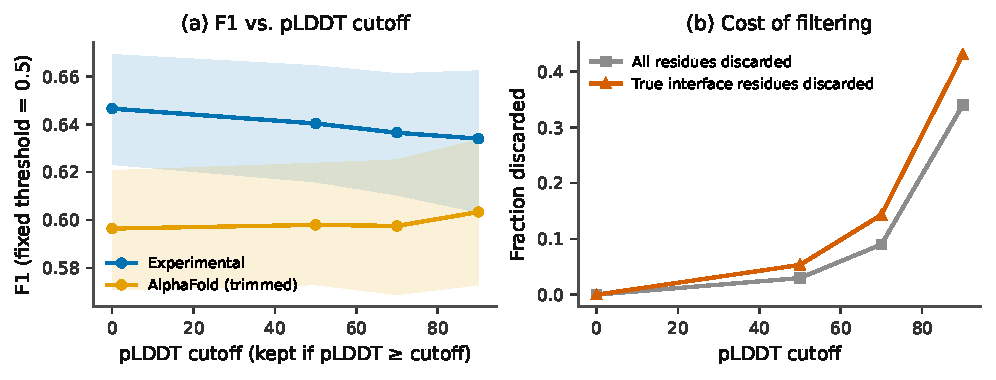
\includegraphics[width=\textwidth]{figures/fig7_plddt_filtering.pdf}
\caption{(a) F1 at a fixed 0.5 probability threshold vs.\ pLDDT cutoff, both
inputs, with 95\% chain-resampled bootstrap CIs. (b) Fraction of all
residues, and of true interface residues specifically, discarded at each
cutoff (identical for both inputs, since pLDDT is a property of the
AlphaFold model, not of which input is scored).}
\label{fig:filtering}
\end{figure}

\begin{table}[t]
\centering
\footnotesize
@@FILTER_TABLE@@
\caption{Precision/recall/F1 (fixed 0.5 threshold) by pLDDT cutoff, both
inputs, with 95\% chain-resampled bootstrap CIs. Post-hoc, exploratory
(Section~\ref{sec:filtering}).}
\label{tab:filtering}
\end{table}

\subsection{Post-hoc checks added after review (exploratory)}
\label{sec:review}

The checks in this subsection were chosen after every result above was known,
in response to peer review (Section~\ref{sec:prespec}). They test the
robustness and interpretation of the pre-specified results and do not
replace them. The paired bootstrap for the filtering analysis, added for the
same reason, is reported with that analysis in Section~\ref{sec:filtering}.

\textbf{Self-templating.} Could AlphaFold DB have used a chain's own
experimental structure as a template? @@TW_BEFORE_N@@ of the @@N_LABELED@@
chains were released before their AlphaFold model was generated, so they
could in principle have been templates for it. This is an upper bound,
because the template database predates the model. The remaining
@@TW_AFTER_N@@ chains cannot have been. Among those (@@TW_AFTER_NS@@ with
defined metrics), the median paired AUPR difference was @@TW_AFTER_MEDIAN@@
(95\% CI @@TW_AFTER_CI@@, $p @@TW_AFTER_P@@$), versus @@TW_BEFORE_MEDIAN@@
(CI @@TW_BEFORE_CI@@, $p @@TW_BEFORE_P@@$) among the @@TW_BEFORE_NS@@ that could have been. The
gap is therefore present without any possibility of self-templating. Its
point estimate is larger in that subgroup, consistent with self-templating
narrowing the gap where it was possible, but the two subgroups were not
formally compared.

\textbf{Shift vs.\ error.} A refit of the Section~\ref{sec:error}
regression design with the signed error
$|p_{\mathrm{AF}} - y| - |p_{\mathrm{exp}} - y|$ as the outcome
(Table~\ref{tab:regcompare}) separates how much a prediction moves from
whether it moves away from the truth. On average AlphaFold-input
predictions are slightly further from the true label (mean
@@ERR_MEAN@@, CI @@ERR_MEAN_CI@@; further for @@ERR_FRAC_WORSE@@ of
residues). Lower pLDDT (coefficient @@ERR_PLDDT_COEF@@, $p @@ERR_PLDDT_P@@$)
and higher local RMSD (@@ERR_RMSD_COEF@@, $p @@ERR_RMSD_P@@$) are both
associated with AlphaFold input being further from the truth, not merely
with a change. Solvent exposure, the strongest correlate of the shift, is not
associated with the signed error (@@ERR_RSA_COEF@@, $p @@ERR_RSA_P@@$).
Exposed residues' predictions move more between inputs, but not
systematically in the wrong direction. This model's $R^2$ is lower still
(@@ERR_R2@@): these covariates identify where errors concentrate, not most of
the residue-level variation.

\begin{table}[t]
\centering
\small
@@REG_COMPARISON_TABLE@@
\caption{Post-hoc. The regression design of Table~\ref{tab:regression}
(same @@REG_N@@ residues, cluster-robust standard errors by chain) with the
pre-specified outcome (left) and the signed error (right; positive when the
AlphaFold-input prediction is further from the true label $y$).}
\label{tab:regcompare}
\end{table}

\textbf{Pooled vs.\ per-chain gap.} Two checks apportion the
pooled-vs.-median difference left unexplained by chain length. Removing the @@PV_TRIM_NREMOVED@@ chains
(@@PV_TRIM_PCT@@) with the largest per-chain drops roughly halves the pooled
gap, from @@POOLED_AUPR_DIFF@@ (CI @@PV_ALL_CI@@) to @@PV_TRIM_GAP@@ (CI
@@PV_TRIM_CI@@). That remainder still exceeds the remaining chains' mean
per-chain drop (@@PV_TRIM_MEAN@@). Replacing each chain's scores by their
within-chain ranks, which removes differences in score calibration between
chains, leaves a pooled gap of @@PV_RANK_GAP@@ (CI @@PV_RANK_CI@@). Rank-based
pooled AUPR is on a different scale from the raw one, so this does not
measure a calibration share. It does show that the pooled gap is not mainly
a calibration artifact: it persists when only within-chain rankings are
compared. The large pooled gap is thus driven substantially, but not
entirely, by the right tail of per-chain drops. (Removing chains selected
on their drop is a diagnostic, not an unbiased estimate.)

\textbf{Flagged chains and extreme local RMSD.} The residue mappings of
the geometrically flagged chains are only slightly less clean than those
of the unflagged chains. @@FA_FLAG_FALLBACK@@ of
@@FA_FLAG_N@@ flagged chains used the fallback alignment, versus
@@FA_UNFLAG_FALLBACK@@ of @@FA_UNFLAG_N@@ unflagged chains;
@@FA_FLAG_MUT@@ versus @@FA_UNFLAG_MUT@@ had at least one sequence mismatch.
Mean mapped identity was @@FA_FLAG_MEANID@@ versus @@FA_UNFLAG_MEANID@@
(Mann--Whitney $p @@FA_P@@$). Mapping problems may contribute for a few
flagged chains but do not characterize the group. Nearly all residues with extreme local RMSD in
Fig.~\ref{fig:regression}a
(@@EX_NRES_FLAGGED@@ of the @@EX_NRES@@ residues above @@EX_THRESH@@\,\r{A},
in @@EX_NCHAINS_FLAGGED@@ of @@EX_NCHAINS@@ chains) belong to geometrically
flagged chains, @@EX_NCHAINS_SIFTS_EXACT@@ of which were mapped by SIFTS with
100\% sequence identity to the AlphaFold model. This makes residue-register
errors an unlikely explanation for most of them, though it does not rule
them out for individual chains.

\section{Discussion}

In practical terms, PeSTo's accuracy cost from using an AlphaFold structure
instead of an experimental one is real, directionally consistent, and
statistically unambiguous, but modest for a typical chain: a median AUPR
difference around @@PRIMARY_MEDIAN@@ on a 0--1 scale is a small-to-moderate
effect, not a collapse in accuracy, and Fig.~\ref{fig:phase7primary}a shows
most chains clustering close to the identity line, with AlphaFold input
actually scoring higher for @@PCT_AF_BETTER@@ of chains. The pooled-residue
comparison (@@POOLED_AUPR_EXP@@ vs.\ @@POOLED_AUPR_AF@@) suggests a larger
gap. Post-hoc checks (Section~\ref{sec:review}) attribute much of that difference to a right-skewed
minority of chains with large drops: removing the @@PV_TRIM_PCT@@ with the
largest drops roughly halves it. The remainder reflects pooled AUPR ranking
residues from all chains together, rather than averaging per-chain values
(Section~\ref{sec:review}).
Reporting the per-chain median alongside the pooled number avoids
overstating the typical case.

This study's numbers are not directly comparable to Yuan et al.'s
ESMFold-based benchmark (median per-protein AUPR 0.797 to 0.691)
\cite{yuan2024}: the structure predictor, the test set, the leakage control,
and the interface definition all differ, and only the direction of the effect
-- a real accuracy cost from using a predicted structure -- is expected to
generalize between the two studies, not the magnitude. AlphaFold's average
accuracy is generally reported as higher than ESMFold's \cite{lin2023}, which
is at least directionally consistent with this study's smaller median
per-chain gap, but the two benchmarks differ in enough other respects that
this is a plausible reading of the comparison, not a controlled one.

The error analysis in Section~\ref{sec:error} indicates where the gap
concentrates, rather than a diffuse ``AlphaFold structures are worse''
pattern: the per-residue cost is largest where AlphaFold itself reports low
confidence and where the local backbone geometry diverges from the
experimental structure, and these two signals carry partly independent
information (low collinearity despite both tracking the same underlying
divergence). A post-hoc refit on the signed error (Section~\ref{sec:review}) shows that both signals
also mark where AlphaFold-input predictions move \emph{away} from the true
label, not merely where they change. Solvent exposure is the strongest
correlate of how much a prediction changes, which is unsurprising for a
method whose interface calls are made on the protein surface, but it is not
associated with the direction of the error. These are associations, and the
covariates explain only a small fraction of residue-level variation. Association with a continuous shift is also not the same as a useful
deployment rule. Section~\ref{sec:filtering}'s direct test of the natural
follow-on idea -- discard low-pLDDT residues before trusting AlphaFold-input
predictions -- found limited practical benefit at a fixed threshold:
AlphaFold-input F1 changed by only @@FILTER_AF_F1_GAIN@@ from no filtering to
the strictest cutoff, while @@FILTER_FRAC_POS_DISCARDED_MAX@@ of the true
interface residues were discarded. pLDDT is a real, independent correlate of
where predictions shift the most; that is a weaker and more qualified claim
than a validated confidence-based filter, and this paper does not claim the
latter.

\section{Limitations}

\begin{itemize}[nosep,leftmargin=1.4em]
\item \textbf{Template and MSA information in the AlphaFold models.} The
release-date filter guarantees that the experimental structures postdate
AlphaFold2's training data, not that they postdate the structural templates
available when the AlphaFold DB models were generated (all models here are
version @@AF_MODEL_VERSIONS@@, created @@AF_MODEL_CREATED_RANGE@@ according
to the API metadata). An experimental structure, or a close homolog,
released before its model was generated could have served as a template for
that model. That would make the AlphaFold input more similar to the
experimental structure and bias the measured gap toward zero. The exact
template cutoff is not recorded in the cached metadata. The post-hoc check
in Section~\ref{sec:review} shows the gap is present among the
@@TW_AFTER_N@@ chains released after their model was generated, which rules
out self-templating for that subgroup, but not templating on earlier close
homologs.
\item \textbf{Temporal and compositional skew.} Leakage filtering removed
@@OVERLAP_PCT@@ of the non-redundant representatives. The remaining set is,
by construction, made of proteins dissimilar to PeSTo's training data, and
results may not transfer to well-studied families. It is also strongly
skewed toward chains released in 2021 or later (release dates
@@PRIMARY_RELEASE_RANGE@@; Supplementary Table~\ref{tab:releaseyear}):
almost no representative released in 2018--2020 survives the filter, which
suggests PeSTo's training-data snapshot extends to roughly 2020--2021, later
than AlphaFold2's cutoff.
\item \textbf{Leakage definition.} Leakage was assessed by sequence identity
alone, and a hit counted only if its alignment covered at least
@@CLUSTER_MIN_COVERAGE@@ of both sequences. Homology confined to one domain
of a multi-domain chain, or structural similarity without detectable
sequence identity, is therefore not excluded.
\item \textbf{Dataset scope.} Only X-ray structures at or better than
@@RESOLUTION_CUTOFF@@\,\r{A} were used. @@N_NONIDENTICAL@@ chains differ from
their AlphaFold model's sequence at one or more mapped positions (identity
$\geq$@@MAPPING_VALIDATION_IDENTITY@@ was allowed, to retain engineered
constructs), so for these the two inputs differ slightly in sequence as well
as structure. The @@MIN_CHAIN_LENGTH@@-residue length filter applies to the
expressed entity, not to the resolved coordinates. Some analyzed chains are
therefore short resolved fragments, including the @@N_EXCLUDED@@ chains that
are entirely interface.
\item \textbf{Bound vs.\ unbound conformations.} All experimental structures
here are bound (holo) structures taken from complexes; a protein's shape can
change somewhat upon binding, and this study cannot separate that ordinary
conformational change from AlphaFold-specific structural error. A planned
comparison against independently solved unbound (apo) structures was not
run.
\item \textbf{Shift rather than error.} The pre-specified regression
outcome $|p_{\mathrm{AF}} - p_{\mathrm{exp}}|$ measures how much a
residue's prediction changes between inputs, not whether the AlphaFold-input
prediction is worse. The signed-error refit that addresses this (Section~\ref{sec:review}) is post-hoc,
and both models have low $R^2$.
\item \textbf{Deferred comparisons.} The untrimmed, full-length AlphaFold
model (as opposed to the same model trimmed to the experimentally observed
range) and the leakage-sensitivity subsets at looser identity thresholds
were not run; the trimmed-model result reported here should not be read as
characterizing performance on a full-length AlphaFold model used without any
trimming.
\item \textbf{Single predictor, single confidence signal.} All results are
specific to PeSTo; whether they generalize to ScanNet \cite{tubiana2022} or
other residue-level interface predictors such as GPSite \cite{yuan2024} or
MaSIF-site \cite{gainza2020} is untested here. (HIGH-PPI \cite{gao2023}
primarily predicts whether two proteins interact, so it is a less direct
comparator.) Only pLDDT was used as AlphaFold's confidence signal; AlphaFold
DB also provides predicted aligned error (PAE) for these monomer models, but
PAE was outside this study's scope.
\item \textbf{Monomeric AlphaFold models.} Every AlphaFold structure used here
is a single-chain model; no multi-chain (complex) AlphaFold prediction was
evaluated, so this study speaks to isolated-chain structure quality, not to
whether an AlphaFold-predicted complex's own interface would look different.
\end{itemize}

\section{Future Work}

The deferred comparisons noted above -- the untrimmed full-length AlphaFold
model, the unbound (apo) structures, and the leakage-sensitivity subsets at
looser identity thresholds -- remain natural next steps and require no new
method, only additional runs of the existing pipeline.
Section~\ref{sec:filtering} found that simply \emph{discarding} low-pLDDT
residues at a fixed threshold recovers little of the measured accuracy cost,
which is itself informative: it suggests the useful information in pLDDT is
more continuous than a hard cutoff can exploit. A pLDDT-\emph{aware}
fine-tuning of PeSTo -- adding pLDDT as an extra per-residue input channel,
training on a mixed set of experimental structures (pLDDT fixed at 100) and
AlphaFold structures (their real pLDDT) -- remains a plausible next step,
since a trained model could in principle learn a more graded use of the
signal than any fixed cutoff; but Section~\ref{sec:filtering} means this
should be treated as an open question to test, not a predicted win.

\section*{Code and Data Availability}

All code, the analysis plans, and the scripts that regenerate every number,
table, and figure in this paper from the pipeline's outputs are available at
@@REPO_URL@@. Supplementary Table~S1, listing every chain in the primary
benchmark set with its UniProt accession, assembly, mapping method, flag
status, per-chain AUPRs, and whether it enters the per-chain analyses, is
@@CHAIN_LIST_FILE@@ in that repository. The structure rendering in
Fig.~\ref{fig:structure} was produced with PyMOL (open-source build, version
@@PYMOL_VERSION@@) \cite{pymol} by \texttt{scripts/render\_example\_chain.py}.
Input data are public: PDB entries via PDBe, AlphaFold DB models via the
AlphaFold DB API, and PeSTo's model and dataset splits via its GitHub
repository.

\section*{AI Assistance Statement}

This project made substantial use of AI assistance, and we describe it here
so that readers can judge the work accordingly. The research question, the
original project proposal, and the decisions that shaped the study (scope,
leakage policy, which analyses to run, and how to respond to review) are the
author's. Claude Code, an AI coding assistant developed by Anthropic and
running Claude large language models, was used throughout, under the
author's direction, for:
\begin{itemize}[nosep,leftmargin=1.4em]
\item writing the data pipeline, analysis code, and tests in the
accompanying repository, and running them;
\item drafting the written analysis plans and this manuscript's text,
figures, and tables, which the author reviewed and revised;
\item checking the manuscript against the pipeline's outputs, and checking
quoted literature values and citation metadata against the original sources
and Crossref.
\end{itemize}
A separate Claude instance, given only the compiled PDF, also produced a
critical review of an earlier draft. Its points were checked against the
repository before being accepted, disputed, or acted on. The
analyses in Section~\ref{sec:review}, and the paired bootstrap in
Section~\ref{sec:filtering}, originated from that review.

Several safeguards limit the risk of AI-introduced errors. Every number in
the paper is generated by a script from the pipeline's own outputs rather
than typed by hand. All analysis code has automated tests. The analysis plans
and full version history are public in the repository. The AI tool is not
listed as an author because it cannot take responsibility for the work. The
author takes full responsibility for the content of this paper, including any
errors.

\section*{Funding}

This work received no funding.

\bibliographystyle{plain}
\begin{thebibliography}{99}

\bibitem{zhang2024} Zhang, J., Durham, J., Cong, Q. Revolutionizing
protein--protein interaction prediction with deep learning. \emph{Curr Opin
Struct Biol} \textbf{85}, 102775 (2024).
\url{https://doi.org/10.1016/j.sbi.2024.102775}

\bibitem{jumper2021} Jumper, J.\ et al.\ Highly accurate protein structure
prediction with AlphaFold. \emph{Nature} \textbf{596}, 583--589 (2021).
\url{https://doi.org/10.1038/s41586-021-03819-2}

\bibitem{varadi2024} Varadi, M.\ et al.\ AlphaFold Protein Structure Database
in 2024: providing structure coverage for over 214 million protein sequences.
\emph{Nucleic Acids Res} \textbf{52}, D368--D375 (2024).
\url{https://doi.org/10.1093/nar/gkad1011}

\bibitem{afdbplddt} EMBL-EBI. pLDDT: understanding local confidence.
AlphaFold online training course.
\url{https://www.ebi.ac.uk/training/online/courses/alphafold/inputs-and-outputs/evaluating-alphafolds-predicted-structures-using-confidence-scores/plddt-understanding-local-confidence/}
(accessed 2026-10-01).

\bibitem{krapp2023} Krapp, L.F., Abriata, L.A., Cort\'es Rodr\'iguez, F.\ et
al.\ PeSTo: parameter-free geometric deep learning for accurate prediction of
protein binding interfaces. \emph{Nat Commun} \textbf{14}, 2175 (2023).
\url{https://doi.org/10.1038/s41467-023-37701-8}

\bibitem{tubiana2022} Tubiana, J., Schneidman-Duhovny, D., Wolfson, H.J.
ScanNet: an interpretable geometric deep learning model for structure-based
protein binding site prediction. \emph{Nat Methods} \textbf{19}, 730--739
(2022). \url{https://doi.org/10.1038/s41592-022-01490-7}

\bibitem{terwilliger2024} Terwilliger, T.C.\ et al.\ AlphaFold predictions are
valuable hypotheses and accelerate but do not replace experimental structure
determination. \emph{Nat Methods} \textbf{21}, 110--116 (2024).
\url{https://doi.org/10.1038/s41592-023-02087-4}

\bibitem{yuan2024} Yuan, Q.\ et al.\ Genome-scale annotation of protein
binding sites via language model and geometric deep learning. \emph{eLife}
\textbf{13}, RP93695 (2024). \url{https://doi.org/10.7554/eLife.93695}

\bibitem{lin2023} Lin, Z.\ et al.\ Evolutionary-scale prediction of
atomic-level protein structure with a language model. \emph{Science}
\textbf{379}, 1123--1130 (2023). \url{https://doi.org/10.1126/science.ade2574}

\bibitem{krissinel2007} Krissinel, E., Henrick, K. Inference of macromolecular
assemblies from crystalline state. \emph{J Mol Biol} \textbf{372}, 774--797
(2007). \url{https://doi.org/10.1016/j.jmb.2007.05.022}

\bibitem{gao2023} Gao, Z., Jiang, C., Zhang, J.\ et al.\ Hierarchical graph
learning for protein--protein interaction. \emph{Nat Commun} \textbf{14}, 1093
(2023). \url{https://doi.org/10.1038/s41467-023-36736-1}

\bibitem{steinegger2017} Steinegger, M., S\"oding, J. MMseqs2 enables
sensitive protein sequence searching for the analysis of massive data sets.
\emph{Nat Biotechnol} \textbf{35}, 1026--1028 (2017).
\url{https://doi.org/10.1038/nbt.3988}

\bibitem{velankar2013} Velankar, S.\ et al.\ SIFTS: Structure Integration
with Function, Taxonomy and Sequences resource. \emph{Nucleic Acids Res}
\textbf{41}, D483--D489 (2013). \url{https://doi.org/10.1093/nar/gks1258}

\bibitem{kunzmann2018} Kunzmann, P., Hamacher, K. Biotite: a unifying open
source computational biology framework in Python. \emph{BMC Bioinformatics}
\textbf{19}, 346 (2018). \url{https://doi.org/10.1186/s12859-018-2367-z}

\bibitem{shrake1973} Shrake, A., Rupley, J.A. Environment and exposure to
solvent of protein atoms. Lysozyme and insulin. \emph{J Mol Biol}
\textbf{79}, 351--371 (1973).
\url{https://doi.org/10.1016/0022-2836(73)90011-9}

\bibitem{tsai1999} Tsai, J., Taylor, R., Chothia, C., Gerstein, M. The
packing density in proteins: standard radii and volumes. \emph{J Mol Biol}
\textbf{290}, 253--266 (1999). \url{https://doi.org/10.1006/jmbi.1999.2829}

\bibitem{tien2013} Tien, M.Z., Meyer, A.G., Sydykova, D.K., Spielman, S.J.,
Wilke, C.O. Maximum allowed solvent accessibilities of residues in proteins.
\emph{PLoS ONE} \textbf{8}, e80635 (2013).
\url{https://doi.org/10.1371/journal.pone.0080635}

\bibitem{labesse1997} Labesse, G., Colloc'h, N., Pothier, J., Mornon, J.-P.
P-SEA: a new efficient assignment of secondary structure from C$\alpha$ trace
of proteins. \emph{Comput Appl Biosci} \textbf{13}, 291--295 (1997).
\url{https://doi.org/10.1093/bioinformatics/13.3.291}

\bibitem{gainza2020} Gainza, P.\ et al.\ Deciphering interaction fingerprints
from protein molecular surfaces using geometric deep learning. \emph{Nat
Methods} \textbf{17}, 184--192 (2020).
\url{https://doi.org/10.1038/s41592-019-0666-6}

\bibitem{pymol} The PyMOL Molecular Graphics System, open-source version.
Schr\"odinger, LLC. \url{https://github.com/schrodinger/pymol-open-source}

\end{thebibliography}

\appendix
\section*{Appendix: release-year breakdown of the leakage filter}

\renewcommand{\thetable}{S2}
\begin{table}[h]
\centering
\small
@@RELEASE_YEAR_TABLE@@
\caption{Non-redundant representatives by PDB release
year: total, number below the @@SEQ_IDENTITY_CUTOFF@@ identity leakage
threshold, percentage flagged as leakage, and number in the final
@@N_LABELED@@-chain primary benchmark set.}
\label{tab:releaseyear}
\end{table}

\end{document}
